\documentclass[11pt]{article}

    \usepackage[breakable]{tcolorbox}
    \usepackage{parskip} % Stop auto-indenting (to mimic markdown behaviour)
    
    \usepackage{iftex}
    \ifPDFTeX
    	\usepackage[T1]{fontenc}
    	\usepackage{mathpazo}
    \else
    	\usepackage{fontspec}
    \fi

    % Basic figure setup, for now with no caption control since it's done
    % automatically by Pandoc (which extracts ![](path) syntax from Markdown).
    \usepackage{graphicx}
    % Maintain compatibility with old templates. Remove in nbconvert 6.0
    \let\Oldincludegraphics\includegraphics
    % Ensure that by default, figures have no caption (until we provide a
    % proper Figure object with a Caption API and a way to capture that
    % in the conversion process - todo).
    \usepackage{caption}
    \DeclareCaptionFormat{nocaption}{}
    \captionsetup{format=nocaption,aboveskip=0pt,belowskip=0pt}

    \usepackage[Export]{adjustbox} % Used to constrain images to a maximum size
    \adjustboxset{max size={0.9\linewidth}{0.9\paperheight}}
    \usepackage{float}
    \floatplacement{figure}{H} % forces figures to be placed at the correct location
    \usepackage{xcolor} % Allow colors to be defined
    \usepackage{enumerate} % Needed for markdown enumerations to work
    \usepackage{geometry} % Used to adjust the document margins
    \usepackage{amsmath} % Equations
    \usepackage{amssymb} % Equations
    \usepackage{textcomp} % defines textquotesingle
    % Hack from http://tex.stackexchange.com/a/47451/13684:
    \AtBeginDocument{%
        \def\PYZsq{\textquotesingle}% Upright quotes in Pygmentized code
    }
\author{Dorde Antonijevic}
    \usepackage{upquote} % Upright quotes for verbatim code
    \usepackage{eurosym} % defines \euro
    \usepackage[mathletters]{ucs} % Extended unicode (utf-8) support
    \usepackage{fancyvrb} % verbatim replacement that allows latex
    \usepackage{grffile} % extends the file name processing of package graphics 
                         % to support a larger range
    \makeatletter % fix for grffile with XeLaTeX
    \def\Gread@@xetex#1{%
      \IfFileExists{"\Gin@base".bb}%
      {\Gread@eps{\Gin@base.bb}}%
      {\Gread@@xetex@aux#1}%
    }
    \makeatother

    % The hyperref package gives us a pdf with properly built
    % internal navigation ('pdf bookmarks' for the table of contents,
    % internal cross-reference links, web links for URLs, etc.)
    \usepackage{hyperref}
    % The default LaTeX title has an obnoxious amount of whitespace. By default,
    % titling removes some of it. It also provides customization options.
    \usepackage{titling}
    \usepackage{longtable} % longtable support required by pandoc >1.10
    \usepackage{booktabs}  % table support for pandoc > 1.12.2
    \usepackage[inline]{enumitem} % IRkernel/repr support (it uses the enumerate* environment)
    \usepackage[normalem]{ulem} % ulem is needed to support strikethroughs (\sout)
                                % normalem makes italics be italics, not underlines
    \usepackage{mathrsfs}
    

    
    % Colors for the hyperref package
    \definecolor{urlcolor}{rgb}{0,.145,.698}
    \definecolor{linkcolor}{rgb}{.71,0.21,0.01}
    \definecolor{citecolor}{rgb}{.12,.54,.11}

    % ANSI colors
    \definecolor{ansi-black}{HTML}{3E424D}
    \definecolor{ansi-black-intense}{HTML}{282C36}
    \definecolor{ansi-red}{HTML}{E75C58}
    \definecolor{ansi-red-intense}{HTML}{B22B31}
    \definecolor{ansi-green}{HTML}{00A250}
    \definecolor{ansi-green-intense}{HTML}{007427}
    \definecolor{ansi-yellow}{HTML}{DDB62B}
    \definecolor{ansi-yellow-intense}{HTML}{B27D12}
    \definecolor{ansi-blue}{HTML}{208FFB}
    \definecolor{ansi-blue-intense}{HTML}{0065CA}
    \definecolor{ansi-magenta}{HTML}{D160C4}
    \definecolor{ansi-magenta-intense}{HTML}{A03196}
    \definecolor{ansi-cyan}{HTML}{60C6C8}
    \definecolor{ansi-cyan-intense}{HTML}{258F8F}
    \definecolor{ansi-white}{HTML}{C5C1B4}
    \definecolor{ansi-white-intense}{HTML}{A1A6B2}
    \definecolor{ansi-default-inverse-fg}{HTML}{FFFFFF}
    \definecolor{ansi-default-inverse-bg}{HTML}{000000}

    % commands and environments needed by pandoc snippets
    % extracted from the output of `pandoc -s`
    \providecommand{\tightlist}{%
      \setlength{\itemsep}{0pt}\setlength{\parskip}{0pt}}
    \DefineVerbatimEnvironment{Highlighting}{Verbatim}{commandchars=\\\{\}}
    % Add ',fontsize=\small' for more characters per line
    \newenvironment{Shaded}{}{}
    \newcommand{\KeywordTok}[1]{\textcolor[rgb]{0.00,0.44,0.13}{\textbf{{#1}}}}
    \newcommand{\DataTypeTok}[1]{\textcolor[rgb]{0.56,0.13,0.00}{{#1}}}
    \newcommand{\DecValTok}[1]{\textcolor[rgb]{0.25,0.63,0.44}{{#1}}}
    \newcommand{\BaseNTok}[1]{\textcolor[rgb]{0.25,0.63,0.44}{{#1}}}
    \newcommand{\FloatTok}[1]{\textcolor[rgb]{0.25,0.63,0.44}{{#1}}}
    \newcommand{\CharTok}[1]{\textcolor[rgb]{0.25,0.44,0.63}{{#1}}}
    \newcommand{\StringTok}[1]{\textcolor[rgb]{0.25,0.44,0.63}{{#1}}}
    \newcommand{\CommentTok}[1]{\textcolor[rgb]{0.38,0.63,0.69}{\textit{{#1}}}}
    \newcommand{\OtherTok}[1]{\textcolor[rgb]{0.00,0.44,0.13}{{#1}}}
    \newcommand{\AlertTok}[1]{\textcolor[rgb]{1.00,0.00,0.00}{\textbf{{#1}}}}
    \newcommand{\FunctionTok}[1]{\textcolor[rgb]{0.02,0.16,0.49}{{#1}}}
    \newcommand{\RegionMarkerTok}[1]{{#1}}
    \newcommand{\ErrorTok}[1]{\textcolor[rgb]{1.00,0.00,0.00}{\textbf{{#1}}}}
    \newcommand{\NormalTok}[1]{{#1}}
    
    % Additional commands for more recent versions of Pandoc
    \newcommand{\ConstantTok}[1]{\textcolor[rgb]{0.53,0.00,0.00}{{#1}}}
    \newcommand{\SpecialCharTok}[1]{\textcolor[rgb]{0.25,0.44,0.63}{{#1}}}
    \newcommand{\VerbatimStringTok}[1]{\textcolor[rgb]{0.25,0.44,0.63}{{#1}}}
    \newcommand{\SpecialStringTok}[1]{\textcolor[rgb]{0.73,0.40,0.53}{{#1}}}
    \newcommand{\ImportTok}[1]{{#1}}
    \newcommand{\DocumentationTok}[1]{\textcolor[rgb]{0.73,0.13,0.13}{\textit{{#1}}}}
    \newcommand{\AnnotationTok}[1]{\textcolor[rgb]{0.38,0.63,0.69}{\textbf{\textit{{#1}}}}}
    \newcommand{\CommentVarTok}[1]{\textcolor[rgb]{0.38,0.63,0.69}{\textbf{\textit{{#1}}}}}
    \newcommand{\VariableTok}[1]{\textcolor[rgb]{0.10,0.09,0.49}{{#1}}}
    \newcommand{\ControlFlowTok}[1]{\textcolor[rgb]{0.00,0.44,0.13}{\textbf{{#1}}}}
    \newcommand{\OperatorTok}[1]{\textcolor[rgb]{0.40,0.40,0.40}{{#1}}}
    \newcommand{\BuiltInTok}[1]{{#1}}
    \newcommand{\ExtensionTok}[1]{{#1}}
    \newcommand{\PreprocessorTok}[1]{\textcolor[rgb]{0.74,0.48,0.00}{{#1}}}
    \newcommand{\AttributeTok}[1]{\textcolor[rgb]{0.49,0.56,0.16}{{#1}}}
    \newcommand{\InformationTok}[1]{\textcolor[rgb]{0.38,0.63,0.69}{\textbf{\textit{{#1}}}}}
    \newcommand{\WarningTok}[1]{\textcolor[rgb]{0.38,0.63,0.69}{\textbf{\textit{{#1}}}}}
    
    
    % Define a nice break command that doesn't care if a line doesn't already
    % exist.
    \def\br{\hspace*{\fill} \\* }
    % Math Jax compatibility definitions
    \def\gt{>}
    \def\lt{<}
    \let\Oldtex\TeX
    \let\Oldlatex\LaTeX
    \renewcommand{\TeX}{\textrm{\Oldtex}}
    \renewcommand{\LaTeX}{\textrm{\Oldlatex}}
    % Document parameters
    % Document title
    \title{Computational Essay}
    
    
    
    
    
% Pygments definitions
\makeatletter
\def\PY@reset{\let\PY@it=\relax \let\PY@bf=\relax%
    \let\PY@ul=\relax \let\PY@tc=\relax%
    \let\PY@bc=\relax \let\PY@ff=\relax}
\def\PY@tok#1{\csname PY@tok@#1\endcsname}
\def\PY@toks#1+{\ifx\relax#1\empty\else%
    \PY@tok{#1}\expandafter\PY@toks\fi}
\def\PY@do#1{\PY@bc{\PY@tc{\PY@ul{%
    \PY@it{\PY@bf{\PY@ff{#1}}}}}}}
\def\PY#1#2{\PY@reset\PY@toks#1+\relax+\PY@do{#2}}

\expandafter\def\csname PY@tok@w\endcsname{\def\PY@tc##1{\textcolor[rgb]{0.73,0.73,0.73}{##1}}}
\expandafter\def\csname PY@tok@c\endcsname{\let\PY@it=\textit\def\PY@tc##1{\textcolor[rgb]{0.25,0.50,0.50}{##1}}}
\expandafter\def\csname PY@tok@cp\endcsname{\def\PY@tc##1{\textcolor[rgb]{0.74,0.48,0.00}{##1}}}
\expandafter\def\csname PY@tok@k\endcsname{\let\PY@bf=\textbf\def\PY@tc##1{\textcolor[rgb]{0.00,0.50,0.00}{##1}}}
\expandafter\def\csname PY@tok@kp\endcsname{\def\PY@tc##1{\textcolor[rgb]{0.00,0.50,0.00}{##1}}}
\expandafter\def\csname PY@tok@kt\endcsname{\def\PY@tc##1{\textcolor[rgb]{0.69,0.00,0.25}{##1}}}
\expandafter\def\csname PY@tok@o\endcsname{\def\PY@tc##1{\textcolor[rgb]{0.40,0.40,0.40}{##1}}}
\expandafter\def\csname PY@tok@ow\endcsname{\let\PY@bf=\textbf\def\PY@tc##1{\textcolor[rgb]{0.67,0.13,1.00}{##1}}}
\expandafter\def\csname PY@tok@nb\endcsname{\def\PY@tc##1{\textcolor[rgb]{0.00,0.50,0.00}{##1}}}
\expandafter\def\csname PY@tok@nf\endcsname{\def\PY@tc##1{\textcolor[rgb]{0.00,0.00,1.00}{##1}}}
\expandafter\def\csname PY@tok@nc\endcsname{\let\PY@bf=\textbf\def\PY@tc##1{\textcolor[rgb]{0.00,0.00,1.00}{##1}}}
\expandafter\def\csname PY@tok@nn\endcsname{\let\PY@bf=\textbf\def\PY@tc##1{\textcolor[rgb]{0.00,0.00,1.00}{##1}}}
\expandafter\def\csname PY@tok@ne\endcsname{\let\PY@bf=\textbf\def\PY@tc##1{\textcolor[rgb]{0.82,0.25,0.23}{##1}}}
\expandafter\def\csname PY@tok@nv\endcsname{\def\PY@tc##1{\textcolor[rgb]{0.10,0.09,0.49}{##1}}}
\expandafter\def\csname PY@tok@no\endcsname{\def\PY@tc##1{\textcolor[rgb]{0.53,0.00,0.00}{##1}}}
\expandafter\def\csname PY@tok@nl\endcsname{\def\PY@tc##1{\textcolor[rgb]{0.63,0.63,0.00}{##1}}}
\expandafter\def\csname PY@tok@ni\endcsname{\let\PY@bf=\textbf\def\PY@tc##1{\textcolor[rgb]{0.60,0.60,0.60}{##1}}}
\expandafter\def\csname PY@tok@na\endcsname{\def\PY@tc##1{\textcolor[rgb]{0.49,0.56,0.16}{##1}}}
\expandafter\def\csname PY@tok@nt\endcsname{\let\PY@bf=\textbf\def\PY@tc##1{\textcolor[rgb]{0.00,0.50,0.00}{##1}}}
\expandafter\def\csname PY@tok@nd\endcsname{\def\PY@tc##1{\textcolor[rgb]{0.67,0.13,1.00}{##1}}}
\expandafter\def\csname PY@tok@s\endcsname{\def\PY@tc##1{\textcolor[rgb]{0.73,0.13,0.13}{##1}}}
\expandafter\def\csname PY@tok@sd\endcsname{\let\PY@it=\textit\def\PY@tc##1{\textcolor[rgb]{0.73,0.13,0.13}{##1}}}
\expandafter\def\csname PY@tok@si\endcsname{\let\PY@bf=\textbf\def\PY@tc##1{\textcolor[rgb]{0.73,0.40,0.53}{##1}}}
\expandafter\def\csname PY@tok@se\endcsname{\let\PY@bf=\textbf\def\PY@tc##1{\textcolor[rgb]{0.73,0.40,0.13}{##1}}}
\expandafter\def\csname PY@tok@sr\endcsname{\def\PY@tc##1{\textcolor[rgb]{0.73,0.40,0.53}{##1}}}
\expandafter\def\csname PY@tok@ss\endcsname{\def\PY@tc##1{\textcolor[rgb]{0.10,0.09,0.49}{##1}}}
\expandafter\def\csname PY@tok@sx\endcsname{\def\PY@tc##1{\textcolor[rgb]{0.00,0.50,0.00}{##1}}}
\expandafter\def\csname PY@tok@m\endcsname{\def\PY@tc##1{\textcolor[rgb]{0.40,0.40,0.40}{##1}}}
\expandafter\def\csname PY@tok@gh\endcsname{\let\PY@bf=\textbf\def\PY@tc##1{\textcolor[rgb]{0.00,0.00,0.50}{##1}}}
\expandafter\def\csname PY@tok@gu\endcsname{\let\PY@bf=\textbf\def\PY@tc##1{\textcolor[rgb]{0.50,0.00,0.50}{##1}}}
\expandafter\def\csname PY@tok@gd\endcsname{\def\PY@tc##1{\textcolor[rgb]{0.63,0.00,0.00}{##1}}}
\expandafter\def\csname PY@tok@gi\endcsname{\def\PY@tc##1{\textcolor[rgb]{0.00,0.63,0.00}{##1}}}
\expandafter\def\csname PY@tok@gr\endcsname{\def\PY@tc##1{\textcolor[rgb]{1.00,0.00,0.00}{##1}}}
\expandafter\def\csname PY@tok@ge\endcsname{\let\PY@it=\textit}
\expandafter\def\csname PY@tok@gs\endcsname{\let\PY@bf=\textbf}
\expandafter\def\csname PY@tok@gp\endcsname{\let\PY@bf=\textbf\def\PY@tc##1{\textcolor[rgb]{0.00,0.00,0.50}{##1}}}
\expandafter\def\csname PY@tok@go\endcsname{\def\PY@tc##1{\textcolor[rgb]{0.53,0.53,0.53}{##1}}}
\expandafter\def\csname PY@tok@gt\endcsname{\def\PY@tc##1{\textcolor[rgb]{0.00,0.27,0.87}{##1}}}
\expandafter\def\csname PY@tok@err\endcsname{\def\PY@bc##1{\setlength{\fboxsep}{0pt}\fcolorbox[rgb]{1.00,0.00,0.00}{1,1,1}{\strut ##1}}}
\expandafter\def\csname PY@tok@kc\endcsname{\let\PY@bf=\textbf\def\PY@tc##1{\textcolor[rgb]{0.00,0.50,0.00}{##1}}}
\expandafter\def\csname PY@tok@kd\endcsname{\let\PY@bf=\textbf\def\PY@tc##1{\textcolor[rgb]{0.00,0.50,0.00}{##1}}}
\expandafter\def\csname PY@tok@kn\endcsname{\let\PY@bf=\textbf\def\PY@tc##1{\textcolor[rgb]{0.00,0.50,0.00}{##1}}}
\expandafter\def\csname PY@tok@kr\endcsname{\let\PY@bf=\textbf\def\PY@tc##1{\textcolor[rgb]{0.00,0.50,0.00}{##1}}}
\expandafter\def\csname PY@tok@bp\endcsname{\def\PY@tc##1{\textcolor[rgb]{0.00,0.50,0.00}{##1}}}
\expandafter\def\csname PY@tok@fm\endcsname{\def\PY@tc##1{\textcolor[rgb]{0.00,0.00,1.00}{##1}}}
\expandafter\def\csname PY@tok@vc\endcsname{\def\PY@tc##1{\textcolor[rgb]{0.10,0.09,0.49}{##1}}}
\expandafter\def\csname PY@tok@vg\endcsname{\def\PY@tc##1{\textcolor[rgb]{0.10,0.09,0.49}{##1}}}
\expandafter\def\csname PY@tok@vi\endcsname{\def\PY@tc##1{\textcolor[rgb]{0.10,0.09,0.49}{##1}}}
\expandafter\def\csname PY@tok@vm\endcsname{\def\PY@tc##1{\textcolor[rgb]{0.10,0.09,0.49}{##1}}}
\expandafter\def\csname PY@tok@sa\endcsname{\def\PY@tc##1{\textcolor[rgb]{0.73,0.13,0.13}{##1}}}
\expandafter\def\csname PY@tok@sb\endcsname{\def\PY@tc##1{\textcolor[rgb]{0.73,0.13,0.13}{##1}}}
\expandafter\def\csname PY@tok@sc\endcsname{\def\PY@tc##1{\textcolor[rgb]{0.73,0.13,0.13}{##1}}}
\expandafter\def\csname PY@tok@dl\endcsname{\def\PY@tc##1{\textcolor[rgb]{0.73,0.13,0.13}{##1}}}
\expandafter\def\csname PY@tok@s2\endcsname{\def\PY@tc##1{\textcolor[rgb]{0.73,0.13,0.13}{##1}}}
\expandafter\def\csname PY@tok@sh\endcsname{\def\PY@tc##1{\textcolor[rgb]{0.73,0.13,0.13}{##1}}}
\expandafter\def\csname PY@tok@s1\endcsname{\def\PY@tc##1{\textcolor[rgb]{0.73,0.13,0.13}{##1}}}
\expandafter\def\csname PY@tok@mb\endcsname{\def\PY@tc##1{\textcolor[rgb]{0.40,0.40,0.40}{##1}}}
\expandafter\def\csname PY@tok@mf\endcsname{\def\PY@tc##1{\textcolor[rgb]{0.40,0.40,0.40}{##1}}}
\expandafter\def\csname PY@tok@mh\endcsname{\def\PY@tc##1{\textcolor[rgb]{0.40,0.40,0.40}{##1}}}
\expandafter\def\csname PY@tok@mi\endcsname{\def\PY@tc##1{\textcolor[rgb]{0.40,0.40,0.40}{##1}}}
\expandafter\def\csname PY@tok@il\endcsname{\def\PY@tc##1{\textcolor[rgb]{0.40,0.40,0.40}{##1}}}
\expandafter\def\csname PY@tok@mo\endcsname{\def\PY@tc##1{\textcolor[rgb]{0.40,0.40,0.40}{##1}}}
\expandafter\def\csname PY@tok@ch\endcsname{\let\PY@it=\textit\def\PY@tc##1{\textcolor[rgb]{0.25,0.50,0.50}{##1}}}
\expandafter\def\csname PY@tok@cm\endcsname{\let\PY@it=\textit\def\PY@tc##1{\textcolor[rgb]{0.25,0.50,0.50}{##1}}}
\expandafter\def\csname PY@tok@cpf\endcsname{\let\PY@it=\textit\def\PY@tc##1{\textcolor[rgb]{0.25,0.50,0.50}{##1}}}
\expandafter\def\csname PY@tok@c1\endcsname{\let\PY@it=\textit\def\PY@tc##1{\textcolor[rgb]{0.25,0.50,0.50}{##1}}}
\expandafter\def\csname PY@tok@cs\endcsname{\let\PY@it=\textit\def\PY@tc##1{\textcolor[rgb]{0.25,0.50,0.50}{##1}}}

\def\PYZbs{\char`\\}
\def\PYZus{\char`\_}
\def\PYZob{\char`\{}
\def\PYZcb{\char`\}}
\def\PYZca{\char`\^}
\def\PYZam{\char`\&}
\def\PYZlt{\char`\<}
\def\PYZgt{\char`\>}
\def\PYZsh{\char`\#}
\def\PYZpc{\char`\%}
\def\PYZdl{\char`\$}
\def\PYZhy{\char`\-}
\def\PYZsq{\char`\'}
\def\PYZdq{\char`\"}
\def\PYZti{\char`\~}
% for compatibility with earlier versions
\def\PYZat{@}
\def\PYZlb{[}
\def\PYZrb{]}
\makeatother


    % For linebreaks inside Verbatim environment from package fancyvrb. 
    \makeatletter
        \newbox\Wrappedcontinuationbox 
        \newbox\Wrappedvisiblespacebox 
        \newcommand*\Wrappedvisiblespace {\textcolor{red}{\textvisiblespace}} 
        \newcommand*\Wrappedcontinuationsymbol {\textcolor{red}{\llap{\tiny$\m@th\hookrightarrow$}}} 
        \newcommand*\Wrappedcontinuationindent {3ex } 
        \newcommand*\Wrappedafterbreak {\kern\Wrappedcontinuationindent\copy\Wrappedcontinuationbox} 
        % Take advantage of the already applied Pygments mark-up to insert 
        % potential linebreaks for TeX processing. 
        %        {, <, #, %, $, ' and ": go to next line. 
        %        _, }, ^, &, >, - and ~: stay at end of broken line. 
        % Use of \textquotesingle for straight quote. 
        \newcommand*\Wrappedbreaksatspecials {% 
            \def\PYGZus{\discretionary{\char`\_}{\Wrappedafterbreak}{\char`\_}}% 
            \def\PYGZob{\discretionary{}{\Wrappedafterbreak\char`\{}{\char`\{}}% 
            \def\PYGZcb{\discretionary{\char`\}}{\Wrappedafterbreak}{\char`\}}}% 
            \def\PYGZca{\discretionary{\char`\^}{\Wrappedafterbreak}{\char`\^}}% 
            \def\PYGZam{\discretionary{\char`\&}{\Wrappedafterbreak}{\char`\&}}% 
            \def\PYGZlt{\discretionary{}{\Wrappedafterbreak\char`\<}{\char`\<}}% 
            \def\PYGZgt{\discretionary{\char`\>}{\Wrappedafterbreak}{\char`\>}}% 
            \def\PYGZsh{\discretionary{}{\Wrappedafterbreak\char`\#}{\char`\#}}% 
            \def\PYGZpc{\discretionary{}{\Wrappedafterbreak\char`\%}{\char`\%}}% 
            \def\PYGZdl{\discretionary{}{\Wrappedafterbreak\char`\$}{\char`\$}}% 
            \def\PYGZhy{\discretionary{\char`\-}{\Wrappedafterbreak}{\char`\-}}% 
            \def\PYGZsq{\discretionary{}{\Wrappedafterbreak\textquotesingle}{\textquotesingle}}% 
            \def\PYGZdq{\discretionary{}{\Wrappedafterbreak\char`\"}{\char`\"}}% 
            \def\PYGZti{\discretionary{\char`\~}{\Wrappedafterbreak}{\char`\~}}% 
        } 
        % Some characters . , ; ? ! / are not pygmentized. 
        % This macro makes them "active" and they will insert potential linebreaks 
        \newcommand*\Wrappedbreaksatpunct {% 
            \lccode`\~`\.\lowercase{\def~}{\discretionary{\hbox{\char`\.}}{\Wrappedafterbreak}{\hbox{\char`\.}}}% 
            \lccode`\~`\,\lowercase{\def~}{\discretionary{\hbox{\char`\,}}{\Wrappedafterbreak}{\hbox{\char`\,}}}% 
            \lccode`\~`\;\lowercase{\def~}{\discretionary{\hbox{\char`\;}}{\Wrappedafterbreak}{\hbox{\char`\;}}}% 
            \lccode`\~`\:\lowercase{\def~}{\discretionary{\hbox{\char`\:}}{\Wrappedafterbreak}{\hbox{\char`\:}}}% 
            \lccode`\~`\?\lowercase{\def~}{\discretionary{\hbox{\char`\?}}{\Wrappedafterbreak}{\hbox{\char`\?}}}% 
            \lccode`\~`\!\lowercase{\def~}{\discretionary{\hbox{\char`\!}}{\Wrappedafterbreak}{\hbox{\char`\!}}}% 
            \lccode`\~`\/\lowercase{\def~}{\discretionary{\hbox{\char`\/}}{\Wrappedafterbreak}{\hbox{\char`\/}}}% 
            \catcode`\.\active
            \catcode`\,\active 
            \catcode`\;\active
            \catcode`\:\active
            \catcode`\?\active
            \catcode`\!\active
            \catcode`\/\active 
            \lccode`\~`\~ 	
        }
    \makeatother

    \let\OriginalVerbatim=\Verbatim
    \makeatletter
    \renewcommand{\Verbatim}[1][1]{%
        %\parskip\z@skip
        \sbox\Wrappedcontinuationbox {\Wrappedcontinuationsymbol}%
        \sbox\Wrappedvisiblespacebox {\FV@SetupFont\Wrappedvisiblespace}%
        \def\FancyVerbFormatLine ##1{\hsize\linewidth
            \vtop{\raggedright\hyphenpenalty\z@\exhyphenpenalty\z@
                \doublehyphendemerits\z@\finalhyphendemerits\z@
                \strut ##1\strut}%
        }%
        % If the linebreak is at a space, the latter will be displayed as visible
        % space at end of first line, and a continuation symbol starts next line.
        % Stretch/shrink are however usually zero for typewriter font.
        \def\FV@Space {%
            \nobreak\hskip\z@ plus\fontdimen3\font minus\fontdimen4\font
            \discretionary{\copy\Wrappedvisiblespacebox}{\Wrappedafterbreak}
            {\kern\fontdimen2\font}%
        }%
        
        % Allow breaks at special characters using \PYG... macros.
        \Wrappedbreaksatspecials
        % Breaks at punctuation characters . , ; ? ! and / need catcode=\active 	
        \OriginalVerbatim[#1,codes*=\Wrappedbreaksatpunct]%
    }
    \makeatother

    % Exact colors from NB
    \definecolor{incolor}{HTML}{303F9F}
    \definecolor{outcolor}{HTML}{D84315}
    \definecolor{cellborder}{HTML}{CFCFCF}
    \definecolor{cellbackground}{HTML}{F7F7F7}
    
    % prompt
    \makeatletter
    \newcommand{\boxspacing}{\kern\kvtcb@left@rule\kern\kvtcb@boxsep}
    \makeatother
    \newcommand{\prompt}[4]{
        \ttfamily\llap{{\color{#2}[#3]:\hspace{3pt}#4}}\vspace{-\baselineskip}
    }
    

    
    % Prevent overflowing lines due to hard-to-break entities
    \sloppy 
    % Setup hyperref package
    \hypersetup{
      breaklinks=true,  % so long urls are correctly broken across lines
      colorlinks=true,
      urlcolor=urlcolor,
      linkcolor=linkcolor,
      citecolor=citecolor,
      }
    % Slightly bigger margins than the latex defaults
    
    \geometry{verbose,tmargin=1in,bmargin=1in,lmargin=1in,rmargin=1in}
    
    

\begin{document}
    
    \maketitle
    
    

    
    \hypertarget{simulating-a-dipole-antenna}{%
\section*{Simulating a Dipole
Antenna}\label{simulating-a-dipole-antenna}}

    In this computational essay I will be simulating the output of a dipole
antenna using two rotating opposite charges. The signal will be the
voltage they cause a at a certain point in space, relative to infinitely
far away (V=0). The dipole will be rotating around the origin in 2D
space. The speed of the rotation will determine the frequency of the
measured signal.

    \begin{figure}
\centering
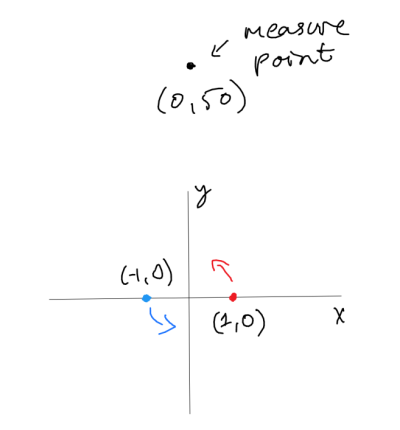
\includegraphics{pics/intro1.png}
\caption{intro1}
\end{figure}

    Defining some values and importing the libraries.

    \begin{tcolorbox}[breakable, size=fbox, boxrule=1pt, pad at break*=1mm,colback=cellbackground, colframe=cellborder]
\prompt{In}{incolor}{123}{\boxspacing}
\begin{Verbatim}[commandchars=\\\{\}]
\PY{k+kn}{import} \PY{n+nn}{numpy} \PY{k}{as} \PY{n+nn}{np}
\PY{k+kn}{import} \PY{n+nn}{matplotlib}\PY{n+nn}{.}\PY{n+nn}{pyplot} \PY{k}{as} \PY{n+nn}{pl}

\PY{n}{e} \PY{o}{=} \PY{l+m+mf}{1.602176634e\PYZhy{}19} \PY{c+c1}{\PYZsh{} absolute value of the charges}
\PY{n}{eps0} \PY{o}{=} \PY{l+m+mf}{8.8541878128e\PYZhy{}12} \PY{c+c1}{\PYZsh{} vacuum permittivity}

\PY{n}{chargesLoc} \PY{o}{=} \PY{n}{np}\PY{o}{.}\PY{n}{array}\PY{p}{(}\PY{p}{[}\PY{p}{[}\PY{o}{\PYZhy{}}\PY{l+m+mi}{1}\PY{p}{,} \PY{l+m+mi}{0}\PY{p}{]}\PY{p}{,} \PY{p}{[}\PY{l+m+mi}{1}\PY{p}{,} \PY{l+m+mi}{0}\PY{p}{]}\PY{p}{]}\PY{p}{)} \PY{c+c1}{\PYZsh{}the position of the charges}
\PY{n}{Q} \PY{o}{=} \PY{p}{[}\PY{o}{\PYZhy{}}\PY{n}{e}\PY{p}{,} \PY{n}{e}\PY{p}{]} \PY{c+c1}{\PYZsh{} value of charges}
\PY{n}{measurePoint} \PY{o}{=} \PY{n}{np}\PY{o}{.}\PY{n}{array}\PY{p}{(}\PY{p}{[}\PY{l+m+mi}{0}\PY{p}{,} \PY{l+m+mi}{50}\PY{p}{]}\PY{p}{)} \PY{c+c1}{\PYZsh{} where the signal is measured}
\end{Verbatim}
\end{tcolorbox}

    The signal will be measured 5000 times a second (sample rate) and this
will also define what a second is.

    \begin{tcolorbox}[breakable, size=fbox, boxrule=1pt, pad at break*=1mm,colback=cellbackground, colframe=cellborder]
\prompt{In}{incolor}{88}{\boxspacing}
\begin{Verbatim}[commandchars=\\\{\}]
\PY{n}{sampleRate} \PY{o}{=} \PY{l+m+mi}{5000} \PY{c+c1}{\PYZsh{} defines time}
\end{Verbatim}
\end{tcolorbox}

    The rotating dipole will produce sinusoidal waves. Lets say we need to
make a wave with a frequency of 100Hz. Then the dipole needs to rotate
once every 1/100 seconds. But a second is 5000 measurements, or frames
lets call them. So 100Hz is one rotation every (1/100) * 5000 frames.

    The function to measure voltage at point in space using the formula for
electric potential from a point charge. \(V = kq/r\)

    \begin{tcolorbox}[breakable, size=fbox, boxrule=1pt, pad at break*=1mm,colback=cellbackground, colframe=cellborder]
\prompt{In}{incolor}{89}{\boxspacing}
\begin{Verbatim}[commandchars=\\\{\}]
\PY{k}{def} \PY{n+nf}{getVoltageAt}\PY{p}{(}\PY{n}{Q}\PY{p}{,} \PY{n}{R}\PY{p}{,} \PY{n}{at}\PY{p}{)}\PY{p}{:}
    \PY{c+c1}{\PYZsh{} Q array of charge values}
    \PY{c+c1}{\PYZsh{} R array of positions of charges}
    \PY{c+c1}{\PYZsh{} at point}
    \PY{n}{k} \PY{o}{=} \PY{l+m+mi}{1} \PY{o}{/} \PY{p}{(}\PY{l+m+mi}{4} \PY{o}{*} \PY{n}{np}\PY{o}{.}\PY{n}{pi} \PY{o}{*} \PY{n}{eps0}\PY{p}{)}
    \PY{k}{return} \PY{n+nb}{sum}\PY{p}{(}\PY{p}{[}\PY{n}{k} \PY{o}{*} \PY{n}{q} \PY{o}{/} \PY{n}{np}\PY{o}{.}\PY{n}{linalg}\PY{o}{.}\PY{n}{norm}\PY{p}{(}\PY{n}{at} \PY{o}{\PYZhy{}} \PY{n}{r}\PY{p}{)} \PY{k}{for} \PY{n}{q}\PY{p}{,} \PY{n}{r} \PY{o+ow}{in} \PY{n+nb}{zip}\PY{p}{(}\PY{n}{Q}\PY{p}{,} \PY{n}{R}\PY{p}{)}\PY{p}{]}\PY{p}{)}
\end{Verbatim}
\end{tcolorbox}

    Now to create a signal. Spin will be a list of values on the form
{[}frequency, how long{]}

    \begin{tcolorbox}[breakable, size=fbox, boxrule=1pt, pad at break*=1mm,colback=cellbackground, colframe=cellborder]
\prompt{In}{incolor}{90}{\boxspacing}
\begin{Verbatim}[commandchars=\\\{\}]
\PY{k}{def} \PY{n+nf}{spinAndMeasure}\PY{p}{(}\PY{n}{Q}\PY{p}{,} \PY{n}{Rch}\PY{p}{,} \PY{n}{spin}\PY{p}{,} \PY{n}{at}\PY{p}{)}\PY{p}{:}
    
    \PY{c+c1}{\PYZsh{} Q charge values}
    \PY{c+c1}{\PYZsh{} Rch position of charges}
    \PY{c+c1}{\PYZsh{} spin  [freq, duration]}
    \PY{c+c1}{\PYZsh{} at \PYZhy{} point of measurement}

    \PY{n}{measured} \PY{o}{=} \PY{p}{[}\PY{p}{]}
    \PY{k}{for} \PY{n}{freq}\PY{p}{,} \PY{n}{t} \PY{o+ow}{in} \PY{n}{spin}\PY{p}{:}

        \PY{n}{dth} \PY{o}{=} \PY{l+m+mi}{2} \PY{o}{*} \PY{n}{np}\PY{o}{.}\PY{n}{pi} \PY{o}{/} \PY{p}{(}\PY{n}{sampleRate} \PY{o}{/} \PY{n}{freq}\PY{p}{)}  \PY{c+c1}{\PYZsh{} dTheta per frame}

        \PY{c+c1}{\PYZsh{} rotation matrix, counter\PYZhy{}clockwise}
        \PY{n}{Rot} \PY{o}{=} \PY{n}{np}\PY{o}{.}\PY{n}{array}\PY{p}{(}\PY{p}{[}\PY{p}{[}\PY{n}{np}\PY{o}{.}\PY{n}{cos}\PY{p}{(}\PY{n}{dth}\PY{p}{)}\PY{p}{,} \PY{o}{\PYZhy{}}\PY{n}{np}\PY{o}{.}\PY{n}{sin}\PY{p}{(}\PY{n}{dth}\PY{p}{)}\PY{p}{]}\PY{p}{,} \PY{p}{[}\PY{n}{np}\PY{o}{.}\PY{n}{sin}\PY{p}{(}\PY{n}{dth}\PY{p}{)}\PY{p}{,} \PY{n}{np}\PY{o}{.}\PY{n}{cos}\PY{p}{(}\PY{n}{dth}\PY{p}{)}\PY{p}{]}\PY{p}{]}\PY{p}{)}

        \PY{c+c1}{\PYZsh{} how many frames/loops}
        \PY{k}{for} \PY{n}{i} \PY{o+ow}{in} \PY{n+nb}{range}\PY{p}{(}\PY{n+nb}{int}\PY{p}{(}\PY{n}{t} \PY{o}{*} \PY{n}{sampleRate}\PY{p}{)}\PY{p}{)}\PY{p}{:} \PY{c+c1}{\PYZsh{} frames = time * sample rate}
            \PY{n}{measured}\PY{o}{.}\PY{n}{append}\PY{p}{(}\PY{n}{getVoltageAt}\PY{p}{(}\PY{n}{Q}\PY{p}{,} \PY{n}{Rch}\PY{p}{,} \PY{n}{at}\PY{p}{)}\PY{p}{)} \PY{c+c1}{\PYZsh{} measure}
            \PY{n}{Rch} \PY{o}{=} \PY{n}{Rot} \PY{o}{@} \PY{n}{Rch} \PY{c+c1}{\PYZsh{} rotate}

    \PY{k}{return} \PY{n}{measured}
\end{Verbatim}
\end{tcolorbox}

    \begin{tcolorbox}[breakable, size=fbox, boxrule=1pt, pad at break*=1mm,colback=cellbackground, colframe=cellborder]
\prompt{In}{incolor}{120}{\boxspacing}
\begin{Verbatim}[commandchars=\\\{\}]
\PY{c+c1}{\PYZsh{} and to visualize a part of the data}

\PY{n}{spin} \PY{o}{=} \PY{n}{np}\PY{o}{.}\PY{n}{array}\PY{p}{(}\PY{p}{[}\PY{p}{[}\PY{l+m+mf}{100.0}\PY{p}{,} \PY{l+m+mf}{2.0}\PY{p}{]}\PY{p}{,} \PY{p}{[}\PY{l+m+mf}{400.0}\PY{p}{,} \PY{l+m+mf}{3.0}\PY{p}{]}\PY{p}{,} \PY{p}{[}\PY{l+m+mf}{200.0}\PY{p}{,} \PY{l+m+mf}{1.0}\PY{p}{]}\PY{p}{]}\PY{p}{)}

\PY{c+c1}{\PYZsh{} switches from 100Hz to 400 at frame 10k}
\PY{n}{data} \PY{o}{=} \PY{n}{spinAndMeasure}\PY{p}{(}\PY{n}{Q}\PY{p}{,} \PY{n}{chargesLoc}\PY{p}{,} \PY{n}{spin}\PY{p}{,} \PY{n}{measurePoint}\PY{p}{)}\PY{p}{[}\PY{l+m+mi}{9900}\PY{p}{:}\PY{l+m+mi}{10100}\PY{p}{]} 

\PY{n}{x} \PY{o}{=} \PY{n+nb}{range}\PY{p}{(}\PY{l+m+mi}{9900}\PY{p}{,} \PY{l+m+mi}{10100}\PY{p}{)}

\PY{n}{pl}\PY{o}{.}\PY{n}{figure}\PY{p}{(}\PY{n}{figsize}\PY{o}{=}\PY{p}{(}\PY{l+m+mi}{8}\PY{p}{,}\PY{l+m+mi}{6}\PY{p}{)}\PY{p}{)}
\PY{n}{pl}\PY{o}{.}\PY{n}{plot}\PY{p}{(}\PY{n}{x}\PY{p}{,} \PY{n}{data}\PY{p}{)}\PY{p}{;} \PY{n}{pl}\PY{o}{.}\PY{n}{ylabel}\PY{p}{(}\PY{l+s+s2}{\PYZdq{}}\PY{l+s+s2}{V}\PY{l+s+s2}{\PYZdq{}}\PY{p}{)}\PY{p}{;} \PY{n}{pl}\PY{o}{.}\PY{n}{xlabel}\PY{p}{(}\PY{l+s+s2}{\PYZdq{}}\PY{l+s+s2}{measurement \PYZsh{}}\PY{l+s+s2}{\PYZdq{}}\PY{p}{)}
\PY{n}{pl}\PY{o}{.}\PY{n}{show}\PY{p}{(}\PY{p}{)}
\end{Verbatim}
\end{tcolorbox}

    \begin{center}
    \adjustimage{max size={0.9\linewidth}{0.9\paperheight}}{output_12_0.png}
    \end{center}
    { \hspace*{\fill} \\}
    
    In spinAndMeasure both contributions to total voltage from q1 and q2
where added simultaneously. Now how would this change if we introduced
the speed of light ? Instead of instantly calculating the voltage, how
about adding a delay, a travel time, to when it arrives at the measure
point. The delay would be distance/speed. So instead of appending values
to measured{[}{]}, each voltage contribution gets a delay attached to
it, and when this time expires the voltage gets added. ``Time'' here is,
of course, frames.

    \begin{tcolorbox}[breakable, size=fbox, boxrule=1pt, pad at break*=1mm,colback=cellbackground, colframe=cellborder]
\prompt{In}{incolor}{121}{\boxspacing}
\begin{Verbatim}[commandchars=\\\{\}]
\PY{k}{def} \PY{n+nf}{spinAndMeasureDelay}\PY{p}{(}\PY{n}{Q}\PY{p}{,} \PY{n}{Rch}\PY{p}{,} \PY{n}{spin}\PY{p}{,} \PY{n}{at}\PY{p}{,} \PY{n}{c}\PY{p}{)}\PY{p}{:}

    \PY{n}{measured} \PY{o}{=} \PY{p}{[}\PY{p}{]}
    \PY{n}{DelayVals} \PY{o}{=} \PY{p}{[}\PY{p}{]}

    \PY{c+c1}{\PYZsh{} every charge gets its own list of [delay, value] variables}
    \PY{k}{for} \PY{n}{i} \PY{o+ow}{in} \PY{n+nb}{range}\PY{p}{(}\PY{n+nb}{len}\PY{p}{(}\PY{n}{Q}\PY{p}{)}\PY{p}{)}\PY{p}{:}
        \PY{n}{DelayVals}\PY{o}{.}\PY{n}{append}\PY{p}{(}\PY{p}{[}\PY{p}{]}\PY{p}{)}

    \PY{k}{for} \PY{n}{freq}\PY{p}{,} \PY{n}{t} \PY{o+ow}{in} \PY{n}{spin}\PY{p}{:}

        \PY{n}{dth} \PY{o}{=} \PY{l+m+mi}{2} \PY{o}{*} \PY{n}{np}\PY{o}{.}\PY{n}{pi} \PY{o}{/} \PY{p}{(}\PY{n}{sampleRate} \PY{o}{/} \PY{n}{freq}\PY{p}{)}  \PY{c+c1}{\PYZsh{} dTheta per frame}

        \PY{c+c1}{\PYZsh{} rotation matrix}
        \PY{n}{Rot} \PY{o}{=} \PY{n}{np}\PY{o}{.}\PY{n}{array}\PY{p}{(}\PY{p}{[}\PY{p}{[}\PY{n}{np}\PY{o}{.}\PY{n}{cos}\PY{p}{(}\PY{n}{dth}\PY{p}{)}\PY{p}{,} \PY{o}{\PYZhy{}}\PY{n}{np}\PY{o}{.}\PY{n}{sin}\PY{p}{(}\PY{n}{dth}\PY{p}{)}\PY{p}{]}\PY{p}{,} \PY{p}{[}\PY{n}{np}\PY{o}{.}\PY{n}{sin}\PY{p}{(}\PY{n}{dth}\PY{p}{)}\PY{p}{,} \PY{n}{np}\PY{o}{.}\PY{n}{cos}\PY{p}{(}\PY{n}{dth}\PY{p}{)}\PY{p}{]}\PY{p}{]}\PY{p}{)}

        \PY{c+c1}{\PYZsh{} how many frames/loops}
        \PY{k}{for} \PY{n}{i} \PY{o+ow}{in} \PY{n+nb}{range}\PY{p}{(}\PY{n+nb}{int}\PY{p}{(}\PY{n}{t} \PY{o}{*} \PY{n}{sampleRate}\PY{p}{)}\PY{p}{)}\PY{p}{:}

            \PY{c+c1}{\PYZsh{} for every q calculate the delay and value of voltage}
            \PY{c+c1}{\PYZsh{} add it to DelayVals}
            \PY{k}{for} \PY{n}{j} \PY{o+ow}{in} \PY{n+nb}{range}\PY{p}{(}\PY{n+nb}{len}\PY{p}{(}\PY{n}{Q}\PY{p}{)}\PY{p}{)}\PY{p}{:}
                \PY{n}{timeDelay} \PY{o}{=} \PY{p}{(}\PY{n}{np}\PY{o}{.}\PY{n}{linalg}\PY{o}{.}\PY{n}{norm}\PY{p}{(}\PY{n}{Rch}\PY{p}{[}\PY{n}{j}\PY{p}{]} \PY{o}{\PYZhy{}} \PY{n}{at}\PY{p}{)} \PY{o}{/} \PY{n}{c}\PY{p}{)} \PY{o}{*} \PY{n}{sampleRate}
                \PY{n}{DelayVals}\PY{p}{[}\PY{n}{j}\PY{p}{]}\PY{o}{.}\PY{n}{append}\PY{p}{(}\PY{p}{[}\PY{n}{timeDelay}\PY{p}{,} \PY{n}{getVoltageAt}\PY{p}{(}\PY{p}{[}\PY{n}{Q}\PY{p}{[}\PY{n}{j}\PY{p}{]}\PY{p}{]}\PY{p}{,} \PY{p}{[}\PY{n}{Rch}\PY{p}{[}\PY{n}{j}\PY{p}{]}\PY{p}{]}\PY{p}{,} \PY{n}{at}\PY{p}{)}\PY{p}{]}\PY{p}{)}

            \PY{n}{measured}\PY{o}{.}\PY{n}{append}\PY{p}{(}\PY{l+m+mf}{0.0}\PY{p}{)}

            \PY{n}{toBeCleaned} \PY{o}{=} \PY{p}{[}\PY{p}{]}

            \PY{k}{for} \PY{n}{val} \PY{o+ow}{in} \PY{n}{DelayVals}\PY{p}{:}
                \PY{k}{for} \PY{n}{l} \PY{o+ow}{in} \PY{n+nb}{range}\PY{p}{(}\PY{n+nb}{len}\PY{p}{(}\PY{n}{val}\PY{p}{)}\PY{p}{)}\PY{p}{:}
                    \PY{k}{if} \PY{n}{val}\PY{p}{[}\PY{n}{l}\PY{p}{]}\PY{p}{[}\PY{l+m+mi}{0}\PY{p}{]} \PY{o}{\PYZlt{}}\PY{o}{=} \PY{l+m+mi}{0}\PY{p}{:}  \PY{c+c1}{\PYZsh{} signal has arrived}
                        \PY{n}{measured}\PY{p}{[}\PY{o}{\PYZhy{}}\PY{l+m+mi}{1}\PY{p}{]} \PY{o}{+}\PY{o}{=} \PY{n}{val}\PY{p}{[}\PY{n}{l}\PY{p}{]}\PY{p}{[}\PY{l+m+mi}{1}\PY{p}{]}  \PY{c+c1}{\PYZsh{} add val to main array}
                        \PY{n}{toBeCleaned}\PY{o}{.}\PY{n}{append}\PY{p}{(}\PY{n}{l}\PY{p}{)}
                    \PY{k}{else}\PY{p}{:}
                        \PY{n}{val}\PY{p}{[}\PY{n}{l}\PY{p}{]}\PY{p}{[}\PY{l+m+mi}{0}\PY{p}{]} \PY{o}{\PYZhy{}}\PY{o}{=} \PY{l+m+mi}{1}  \PY{c+c1}{\PYZsh{} time ticks down}

                \PY{k}{for} \PY{n}{l} \PY{o+ow}{in} \PY{n}{toBeCleaned}\PY{p}{:}
                    \PY{k}{del} \PY{n}{val}\PY{p}{[}\PY{n}{l}\PY{p}{]}
                \PY{n}{toBeCleaned}\PY{o}{.}\PY{n}{clear}\PY{p}{(}\PY{p}{)}

            \PY{n}{Rch} \PY{o}{=} \PY{n}{Rot} \PY{o}{@} \PY{n}{Rch}

    \PY{k}{return} \PY{n}{measured}
\end{Verbatim}
\end{tcolorbox}

    The simulated delay wont be very presise since time here moves in units
of 1 frame, rounded up. So if the initial delay is 0.1 frames thats as
if it were 1. Any effect that delay can have on the measurement is
amplified just a bit. But lets compare this model with the instant one.

    \begin{tcolorbox}[breakable, size=fbox, boxrule=1pt, pad at break*=1mm,colback=cellbackground, colframe=cellborder]
\prompt{In}{incolor}{122}{\boxspacing}
\begin{Verbatim}[commandchars=\\\{\}]
\PY{n}{end}\PY{o}{=}\PY{l+m+mi}{150}

\PY{n}{data1} \PY{o}{=} \PY{n}{spinAndMeasureDelay}\PY{p}{(}\PY{n}{Q}\PY{p}{,} \PY{n}{chargesLoc}\PY{p}{,} \PY{n}{spin}\PY{p}{,} \PY{n}{measurePoint}\PY{p}{,} \PY{l+m+mi}{300\PYZus{}000\PYZus{}000}\PY{p}{)}\PY{p}{[}\PY{p}{:}\PY{n}{end}\PY{p}{]}
\PY{n}{x} \PY{o}{=} \PY{n+nb}{range}\PY{p}{(}\PY{n}{end}\PY{p}{)}

\PY{n}{data2} \PY{o}{=} \PY{n}{spinAndMeasure}\PY{p}{(}\PY{n}{Q}\PY{p}{,} \PY{n}{chargesLoc}\PY{p}{,} \PY{n}{spin}\PY{p}{,} \PY{n}{measurePoint}\PY{p}{)}\PY{p}{[}\PY{p}{:}\PY{n}{end}\PY{p}{]} 

\PY{n}{pl}\PY{o}{.}\PY{n}{figure}\PY{p}{(}\PY{n}{figsize}\PY{o}{=}\PY{p}{(}\PY{l+m+mi}{7}\PY{p}{,} \PY{l+m+mi}{7}\PY{p}{)}\PY{p}{)}
\PY{n}{pl}\PY{o}{.}\PY{n}{subplot}\PY{p}{(}\PY{l+m+mi}{211}\PY{p}{)}
\PY{n}{pl}\PY{o}{.}\PY{n}{plot}\PY{p}{(}\PY{n}{x}\PY{p}{,} \PY{n}{data1}\PY{p}{,} \PY{n}{label}\PY{o}{=}\PY{l+s+s2}{\PYZdq{}}\PY{l+s+s2}{delayed}\PY{l+s+s2}{\PYZdq{}}\PY{p}{)}
\PY{n}{pl}\PY{o}{.}\PY{n}{ylabel}\PY{p}{(}\PY{l+s+s2}{\PYZdq{}}\PY{l+s+s2}{V}\PY{l+s+s2}{\PYZdq{}}\PY{p}{)}\PY{p}{;} \PY{n}{pl}\PY{o}{.}\PY{n}{xlabel}\PY{p}{(}\PY{l+s+s2}{\PYZdq{}}\PY{l+s+s2}{frame \PYZsh{}}\PY{l+s+s2}{\PYZdq{}}\PY{p}{)}\PY{p}{;} \PY{n}{pl}\PY{o}{.}\PY{n}{legend}\PY{p}{(}\PY{p}{)}

\PY{n}{pl}\PY{o}{.}\PY{n}{subplot}\PY{p}{(}\PY{l+m+mi}{212}\PY{p}{)}
\PY{n}{pl}\PY{o}{.}\PY{n}{plot}\PY{p}{(}\PY{n}{x}\PY{p}{,} \PY{n}{data2}\PY{p}{,} \PY{n}{label}\PY{o}{=}\PY{l+s+s2}{\PYZdq{}}\PY{l+s+s2}{instant}\PY{l+s+s2}{\PYZdq{}}\PY{p}{)}
\PY{n}{pl}\PY{o}{.}\PY{n}{ylabel}\PY{p}{(}\PY{l+s+s2}{\PYZdq{}}\PY{l+s+s2}{V}\PY{l+s+s2}{\PYZdq{}}\PY{p}{)}\PY{p}{;} \PY{n}{pl}\PY{o}{.}\PY{n}{xlabel}\PY{p}{(}\PY{l+s+s2}{\PYZdq{}}\PY{l+s+s2}{frame \PYZsh{}}\PY{l+s+s2}{\PYZdq{}}\PY{p}{)}\PY{p}{;} \PY{n}{pl}\PY{o}{.}\PY{n}{legend}\PY{p}{(}\PY{p}{)}
\PY{n}{pl}\PY{o}{.}\PY{n}{show}\PY{p}{(}\PY{p}{)}

\PY{n+nb}{print}\PY{p}{(}\PY{l+s+sa}{f}\PY{l+s+s2}{\PYZdq{}}\PY{l+s+s2}{Delayed value at frame 91: }\PY{l+s+si}{\PYZob{}data1[91]\PYZcb{}}\PY{l+s+s2}{\PYZdq{}}\PY{p}{)}
\PY{n+nb}{print}\PY{p}{(}\PY{l+s+sa}{f}\PY{l+s+s2}{\PYZdq{}}\PY{l+s+s2}{Instant value at frame 90: }\PY{l+s+si}{\PYZob{}data2[90]\PYZcb{}}\PY{l+s+s2}{\PYZdq{}}\PY{p}{)}
\end{Verbatim}
\end{tcolorbox}

    \begin{center}
    \adjustimage{max size={0.9\linewidth}{0.9\paperheight}}{output_16_0.png}
    \end{center}
    { \hspace*{\fill} \\}
    
    \begin{Verbatim}[commandchars=\\\{\}]
Delayed value at frame 91: 3.6993215621436464e-13
Instant value at frame 90: 3.6993215621436464e-13
    \end{Verbatim}

    Practically no difference. Only a frame of delay that frame comes from
rounding up from 0.000833. The charges are 2m away from each other and
the measure point 50m away from their center. This is expected. Now what
if we slow down the speed of light and move the charges and the measure
point a little farther from each other ?

    \begin{tcolorbox}[breakable, size=fbox, boxrule=1pt, pad at break*=1mm,colback=cellbackground, colframe=cellborder]
\prompt{In}{incolor}{105}{\boxspacing}
\begin{Verbatim}[commandchars=\\\{\}]
\PY{n}{chargesLoc} \PY{o}{=} \PY{n}{np}\PY{o}{.}\PY{n}{array}\PY{p}{(}\PY{p}{[}\PY{p}{[}\PY{l+m+mi}{1000}\PY{p}{,} \PY{o}{\PYZhy{}}\PY{l+m+mi}{1000}\PY{p}{]}\PY{p}{,} \PY{p}{[}\PY{o}{\PYZhy{}}\PY{l+m+mi}{1000}\PY{p}{,} \PY{l+m+mi}{1000}\PY{p}{]}\PY{p}{]}\PY{p}{)}
\PY{n}{measurePoint} \PY{o}{=} \PY{n}{np}\PY{o}{.}\PY{n}{array}\PY{p}{(}\PY{p}{[}\PY{l+m+mi}{0}\PY{p}{,} \PY{l+m+mi}{10000}\PY{p}{]}\PY{p}{)}

\PY{n}{a} \PY{o}{=} \PY{l+m+mi}{9800}
\PY{n}{b} \PY{o}{=} \PY{l+m+mi}{10100}

\PY{n}{data1} \PY{o}{=} \PY{n}{spinAndMeasureDelay}\PY{p}{(}\PY{n}{Q}\PY{p}{,} \PY{n}{chargesLoc}\PY{p}{,} \PY{n}{spin}\PY{p}{,} \PY{n}{measurePoint}\PY{p}{,} \PY{l+m+mi}{300\PYZus{}000}\PY{p}{)}\PY{p}{[}\PY{n}{a}\PY{p}{:}\PY{n}{b}\PY{p}{]}
\PY{n}{x} \PY{o}{=} \PY{n+nb}{range}\PY{p}{(}\PY{n}{a}\PY{p}{,} \PY{n}{b}\PY{p}{)}

\PY{n}{data2} \PY{o}{=} \PY{n}{spinAndMeasure}\PY{p}{(}\PY{n}{Q}\PY{p}{,} \PY{n}{chargesLoc}\PY{p}{,} \PY{n}{spin}\PY{p}{,} \PY{n}{measurePoint}\PY{p}{)}\PY{p}{[}\PY{n}{a}\PY{p}{:}\PY{n}{b}\PY{p}{]} 

\PY{n}{pl}\PY{o}{.}\PY{n}{figure}\PY{p}{(}\PY{n}{figsize}\PY{o}{=}\PY{p}{(}\PY{l+m+mi}{7}\PY{p}{,} \PY{l+m+mi}{7}\PY{p}{)}\PY{p}{)}
\PY{n}{pl}\PY{o}{.}\PY{n}{subplot}\PY{p}{(}\PY{l+m+mi}{211}\PY{p}{)}
\PY{n}{pl}\PY{o}{.}\PY{n}{plot}\PY{p}{(}\PY{n}{x}\PY{p}{,} \PY{n}{data1}\PY{p}{,} \PY{n}{label}\PY{o}{=}\PY{l+s+s2}{\PYZdq{}}\PY{l+s+s2}{delayed}\PY{l+s+s2}{\PYZdq{}}\PY{p}{)}
\PY{n}{pl}\PY{o}{.}\PY{n}{ylabel}\PY{p}{(}\PY{l+s+s2}{\PYZdq{}}\PY{l+s+s2}{V}\PY{l+s+s2}{\PYZdq{}}\PY{p}{)}\PY{p}{;} \PY{n}{pl}\PY{o}{.}\PY{n}{xlabel}\PY{p}{(}\PY{l+s+s2}{\PYZdq{}}\PY{l+s+s2}{frame \PYZsh{}}\PY{l+s+s2}{\PYZdq{}}\PY{p}{)}\PY{p}{;} \PY{n}{pl}\PY{o}{.}\PY{n}{legend}\PY{p}{(}\PY{p}{)}

\PY{n}{pl}\PY{o}{.}\PY{n}{subplot}\PY{p}{(}\PY{l+m+mi}{212}\PY{p}{)}
\PY{n}{pl}\PY{o}{.}\PY{n}{plot}\PY{p}{(}\PY{n}{x}\PY{p}{,} \PY{n}{data2}\PY{p}{,} \PY{n}{label}\PY{o}{=}\PY{l+s+s2}{\PYZdq{}}\PY{l+s+s2}{instant}\PY{l+s+s2}{\PYZdq{}}\PY{p}{)}
\PY{n}{pl}\PY{o}{.}\PY{n}{ylabel}\PY{p}{(}\PY{l+s+s2}{\PYZdq{}}\PY{l+s+s2}{V}\PY{l+s+s2}{\PYZdq{}}\PY{p}{)}\PY{p}{;} \PY{n}{pl}\PY{o}{.}\PY{n}{xlabel}\PY{p}{(}\PY{l+s+s2}{\PYZdq{}}\PY{l+s+s2}{frame \PYZsh{}}\PY{l+s+s2}{\PYZdq{}}\PY{p}{)}\PY{p}{;} \PY{n}{pl}\PY{o}{.}\PY{n}{legend}\PY{p}{(}\PY{p}{)}
\PY{n}{pl}\PY{o}{.}\PY{n}{show}\PY{p}{(}\PY{p}{)}
\end{Verbatim}
\end{tcolorbox}

    \begin{center}
    \adjustimage{max size={0.9\linewidth}{0.9\paperheight}}{output_18_0.png}
    \end{center}
    { \hspace*{\fill} \\}
    
    We can see the the delayed version still hasnt caught up to the change
in frequency, and its wave seems quite weird indeed.

    Now how can these rotating charges be used to generate something other
than sine waves? Lets see how their individual signals look like from a
point (0, 50).

    \begin{tcolorbox}[breakable, size=fbox, boxrule=1pt, pad at break*=1mm,colback=cellbackground, colframe=cellborder]
\prompt{In}{incolor}{114}{\boxspacing}
\begin{Verbatim}[commandchars=\\\{\}]
\PY{n}{Q1} \PY{o}{=} \PY{p}{[}\PY{n}{e}\PY{p}{]}
\PY{n}{R1} \PY{o}{=} \PY{n}{np}\PY{o}{.}\PY{n}{array}\PY{p}{(}\PY{p}{[}\PY{l+m+mi}{1}\PY{p}{,} \PY{l+m+mi}{0}\PY{p}{]}\PY{p}{)}

\PY{n}{Q2} \PY{o}{=} \PY{p}{[}\PY{n}{e}\PY{p}{]}
\PY{n}{R2} \PY{o}{=} \PY{n}{np}\PY{o}{.}\PY{n}{array}\PY{p}{(}\PY{p}{[}\PY{l+m+mi}{0}\PY{p}{,} \PY{o}{\PYZhy{}}\PY{l+m+mi}{1}\PY{p}{]}\PY{p}{)}

\PY{n}{freq} \PY{o}{=} \PY{p}{[}\PY{p}{[}\PY{l+m+mi}{100}\PY{p}{,} \PY{l+m+mf}{0.1}\PY{p}{]}\PY{p}{]}

\PY{n}{data1} \PY{o}{=} \PY{n}{spinAndMeasure}\PY{p}{(}\PY{n}{Q1}\PY{p}{,} \PY{n}{R1}\PY{p}{,} \PY{n}{freq}\PY{p}{,} \PY{p}{[}\PY{l+m+mi}{0}\PY{p}{,} \PY{l+m+mi}{50}\PY{p}{]}\PY{p}{)}
\PY{n}{data2} \PY{o}{=} \PY{n}{spinAndMeasure}\PY{p}{(}\PY{n}{Q2}\PY{p}{,} \PY{n}{R2}\PY{p}{,} \PY{n}{freq}\PY{p}{,} \PY{p}{[}\PY{l+m+mi}{0}\PY{p}{,} \PY{l+m+mi}{50}\PY{p}{]}\PY{p}{)}

\PY{n}{x} \PY{o}{=} \PY{n+nb}{range}\PY{p}{(}\PY{n+nb}{len}\PY{p}{(}\PY{n}{data1}\PY{p}{)}\PY{p}{)}

\PY{n}{pl}\PY{o}{.}\PY{n}{subplot}\PY{p}{(}\PY{l+m+mi}{211}\PY{p}{)}
\PY{n}{pl}\PY{o}{.}\PY{n}{plot}\PY{p}{(}\PY{n}{x}\PY{p}{,} \PY{n}{data1}\PY{p}{,} \PY{n}{label}\PY{o}{=}\PY{l+s+sa}{f}\PY{l+s+s2}{\PYZdq{}}\PY{l+s+si}{\PYZob{}R1\PYZcb{}}\PY{l+s+s2}{\PYZdq{}}\PY{p}{)}\PY{p}{;} \PY{n}{pl}\PY{o}{.}\PY{n}{legend}\PY{p}{(}\PY{p}{)}
\PY{n}{pl}\PY{o}{.}\PY{n}{subplot}\PY{p}{(}\PY{l+m+mi}{212}\PY{p}{)}
\PY{n}{pl}\PY{o}{.}\PY{n}{plot}\PY{p}{(}\PY{n}{x}\PY{p}{,} \PY{n}{data2}\PY{p}{,} \PY{n}{label}\PY{o}{=}\PY{l+s+sa}{f}\PY{l+s+s2}{\PYZdq{}}\PY{l+s+si}{\PYZob{}R2\PYZcb{}}\PY{l+s+s2}{\PYZdq{}}\PY{p}{)}\PY{p}{;} \PY{n}{pl}\PY{o}{.}\PY{n}{legend}\PY{p}{(}\PY{p}{)}
\PY{n}{pl}\PY{o}{.}\PY{n}{show}\PY{p}{(}\PY{p}{)}
\end{Verbatim}
\end{tcolorbox}

    \begin{center}
    \adjustimage{max size={0.9\linewidth}{0.9\paperheight}}{output_21_0.png}
    \end{center}
    { \hspace*{\fill} \\}
    
    Now those look like cos and sin functions, respectively. The speed of
rotation can be seen as a scaling factor for the variable inside. If
lets say 100Hz is the standard, call it cos(x), 200Hz would be cos(2x).

So by picking the speed of rotation, and where (more probably when) the
charges start rotating we can produce waves that look like

    \begin{figure}
\centering
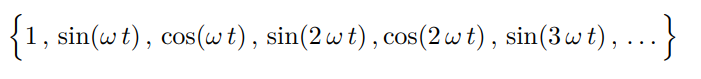
\includegraphics{pics/cossin.png}
\caption{cossin}
\end{figure}

    With linear combinations of these function we can interpolate (more
functions -\textgreater{} more points) any single-valued function on an
interval {[}a, b{]} if we set \(\omega=\frac{2\pi}{b-a}\) and the value
of the charges would then be coefficients in front of the functions.

    


    % Add a bibliography block to the postdoc
    
    
    
\end{document}
